\documentclass{IEEEtran}
\title{Gaussian Process Motion Planning}
\author{Mustafa Mukadam, Xinyan Yan, and Byron Boots\thanks{Mustafa Mukadam, Xinyan Yan, and Byron Boots are affiliated with
the Institute for Robotics and Intelligent Machines, Georgia Institute
of Technology, Atlanta, GA 30332, USA. mmukadam3@gatech.edu
{xinyan.yan,bboots}@cc.gatech.edu. This work was funded in
part by the National Science Foundation, grant number IIS-1464219.}}
\date{}
\usepackage{amsmath,amssymb,amsfonts}
\usepackage{bm}
\usepackage[ruled,linesnumbered,lined]{algorithm2e}
\usepackage{algpseudocode}
\usepackage{mathrsfs}
\usepackage{url}
\usepackage{caption}
\usepackage{graphicx,subfig}
\usepackage{cite}
\begin{document}
\maketitle
\pagestyle{empty}
\thispagestyle{empty}
\textbf{\emph{Abstract}-Motion planning is a fundamental tool in robotics,
used to generate collision-free, smooth, trajectories, while satisfying task-dependent constraints. In this paper, we present a
novel approach to motion planning using Gaussian processes.
In contrast to most existing trajectory optimization algorithms,
which rely on a discrete state parameterization in practice,
we represent the continuous-time trajectory as a sample from
a Gaussian process (GP) generated by a linear time-varying
stochastic differential equation. We then provide a gradient-based optimization technique that optimizes continuous-time
trajectories with respect to a cost functional. By exploiting GP
interpolation, we develop the Gaussian Process Motion Planner
(GPMP), that finds optimal trajectories parameterized by a
small number of states. We benchmark our algorithm against
recent trajectory optimization algorithms by solving 7-DOF
robotic arm planning problems in simulation and validate our
approach on a real 7-DOF WAM arm.}
\section{INTRODUCTION \& RELATED WORK}
Motion planning is a fundamental skill for robots that
aspire to move through an environment without collision
or manipulate objects to achieve some goal. We consider
motion planning from a trajectory optimization perspective,
where we seek to find a trajectory that minimizes a given
cost function while satisfying any given constraints.

A significant amount of previous work has focused on
trajectory optimization and related problems. Khatib [1]
pioneered the idea of potential field where the goal position is
an attractive pole and the obstacles form repulsive fields. Various extensions have been proposed to address problems like
local minimum [2], and ways of modeling the free space [3].
Covariant Hamiltonian Optimization for Motion Planning
(CHOMP) [4], [5] utilizes covariant gradient descent to minimize obstacle and smoothness cost functionals, and a precomputed signed distance field for fast collision checking.
STOMP [6] is a stochastic trajectory optimization method
that can work with non-differentiable constraints by sampling
a series of noisy trajectories. An important drawback of
CHOMP and STOMP is that a large number of trajectory
states are needed to reason about small obstacles or find
feasible solutions when there are many constraints. Multigrid
CHOMP [7] attempts to reduce the computation time of
CHOMP when using a large number of states by starting
with a low-resolution trajectory and gradually increasing the
resolution at each iteration. Finally, TrajOpt [8] formulates
motion planning as sequential quadratic programming. Swept 
volumes are considered to ensure continuous-time safety,
enabling TrajOpt to solve more problems with fewer states.

In this paper, we present a novel Gaussian process (GP)
approach to motion planning. Although, Gaussian processes
[9] have been used for function approximation in many areas
of robotics including supervised learning [10], [11], inverse
dynamics modeling [12], [13], reinforcement learning [14],
path prediction [15], simultaneous localization and mapping [16], [17], state estimation [18]–[20], and controls [21],
to our knowledge they have not been used for motion
planning before.

GPs provide a very natural way to model motion planning
problems with several advantages over previous approaches.
Vector-valued GPs provide a principled way to represent
continuous-time trajectories as functions that map time to
robot states. Smooth trajectories can be represented compactly with only a small number of states, and Gaussian
process regression can be used to query the state of the robot
at any time of interest. Using this insight, we develop the
Gaussian Process Motion Planner (GPMP), a new motion
planning algorithm that optimizes trajectories parameterized
by a small number of states, using Gaussian process interpolation and gradient-based optimization. We evaluate our
algorithm both in simulation and on a 7-DOF Barrett WAM
arm, and we benchmark our approach against several recent
trajectory optimization algorithms.

\section{A GAUSSIAN PROCESS MODEL FOR CONTINUOUS-TIME TRAJECTORIES}
Motion planning traditionally involves finding a smooth,
collision-free trajectory from a start state to a goal state.
Similar to previous approaches [4]–[8], we treat motion planning as an optimization problem and search for a trajectory
that minimizes a predefined cost function (Section III). In
contrast to these previous approaches, which consider finely
discretized discrete time trajectories in practice, we consider
continuous-time trajectories such that the state at time \emph{t} is 

\begin{equation}
\xi(t)=\left\{\xi^d(t)\right\}^D_{d=1} \quad
\xi^d(t)=\left\{\xi^{dr}(t)\right\}^R_{r=1}
\end{equation}
where D is the dimension of the configuration space (number
of joints), and R is the number of variables in each configuration dimension. Here we choose R = 3, specifying joint
positions, velocities, and accelerations, ensuring that our
state is Markovian. Using the Markov property of the state in
the motion prior, defined in Eq. 6 below, allows us to build
an exactly sparse inverse kernel (precision matrix) [16], [22]
useful for efficient optimization and fast GP interpolation
(Section II-B)

Continuous-time trajectories are assumed to be sampled
from a vector-valued Gaussian process (GP):

\begin{equation}
\xi(t)\sim{\emph{$\mathcal{GP}$}}(\mu(t),{\mathcal{K}}(t,t')) \quad 
t_0<t,t'<t_{N+1}
\end{equation}
where $\mu(t)$ is a vector-valued mean function whose components are the functions $\left\{\mu^{dr}{(t)}\right\}^{D,R}_{d=1,r=1}$ and the entries ${\mathcal{K}}(t,t')_{{dr},{d'r'}}$ in the matrix-valued covariance function  ${\mathcal{K}}(t,t')$ corresponding to the covariances between $\xi^{dr}(t)$ and $\xi^{d'r'}(t')$. Based on the definition of vector-valued Gaussian
processes [23], any collection of N states on the trajectory
has a joint Gaussian distribution,

\begin{equation}
\begin{split}
\xi\sim{\mathcal{N}(\mu,\mathcal{K})},\quad \xi=\xi_{1:N}, \quad \mu=\mu_{1:N} \\
\mathcal{K}_{ij}=\mathcal{K}(t_i,t_j),\quad 
t_1\leq{t_i},t_j\leq{t_N}
\end{split}
\end{equation}

The start and goal states, $\xi_0$ and $\xi_{N+1}$, are excluded because
they are fixed. $\xi_i$ denotes the state at time $t_i$.

Reasoning about trajectories with GPs has several advantages. The Gaussian process imposes a prior distribution
on the space of trajectories. Given a fixed set of timeparameterized states, we can condition the GP on those states
to compute the posterior mean at any time of interest:
\begin{gather}
\bar{\xi}(\tau)=\mu(\tau)+\mathcal{K}(\tau)\mathcal{K}^{-1}(\xi-\mu)\\
\mathcal{K}(\tau)=[\mathcal{K}(\tau,t_1) \quad... \quad \mathcal{K}(\tau,t_N)]
\end{gather}
A consequence of GP interpolation is that the trajectory does
not need to be discretized at a high resolution, and trajectory
states do not need to be evenly spaced in time. Additionally,
the posterior mean is the maximum a posteriori interpolation
of the trajectory, and high-frequency interpolation can be
used to generate an executable trajectory or reason about the
cost over the entire trajectory instead of just at the states.
\subsection{Gaussian Processes Generated by Linear Time-Varying
Stochastic Differential Equations}
The choice of prior is an important design consideration
when working with Gaussian processes. In this work, we
consider the Gaussian processes generated by the linear time
varying (LTV) stochastic differential equations (SDEs) [16]:
\begin{equation}
\begin{split}
&\xi'(t)=A(t)\xi(t)+F(t)\omega(t)\\
&\omega(t)\sim{\mathcal{GP}(0,{Q_c\delta(t-t')})},\quad t_0<t,t'<t_{N+1}
\end{split}
\end{equation}
where A(t) are F(t) are time-varying system matrices, $\delta(\cdot)$
is the Dirac delta function, w(t) is the process noise modeled
by a Gaussian process with zero mean, and Qc is a powerspectral density matrix, a hyperparameter that can be set
using data collected on the system [16].

Given the fixed start state $\xi_0$ as the initial condition, and
$\Phi(t, s)$, the state transition matrix that propagates the state
from time s to t, the solution to the SDE is:

\begin{equation}
\tilde{\xi}(t)=\Phi(t,{t_0}){\xi_0}+\int_{t_0}^{t}\Phi(t,s)F(s)\omega(s)ds
\end{equation}
$\tilde{\xi}(t)$ corresponds to a Gaussian process. The mean function
and the covariance function can be obtained from the first
and second moments:

\begin{equation}
\tilde{\mu}(t)=\Phi(t,{t_0}){\xi_0}
\end{equation}

\begin{equation}
\begin{split}
\tilde{\mathcal{K}}(t,t')&=E[(\tilde{\xi}(t)-\tilde{\mu}(t)){(\tilde{\xi}(t')-\tilde{\mu}(t'))}^T]\\
&=\int_{t_0}^{min(t,t')}\Phi(t,s)F(s)Q_c{F(s)}^T{\Phi(t',s)}^Tds
\end{split}
\end{equation}
After considering the end state $\xi_{N+1}$as a noise-free “measurement”, and conditioning $\tilde{\xi}(t)$ on this measurement, we
derive the Gaussian process for the trajectories with fixed
start and end states. The mean and covariance functions are:

\begin{align}
\mu(t)&=\tilde{\mu}_t+\tilde{\mathcal{K}}_{{N+1},t}{\tilde{\mathcal{K}}_{{N+1},{N+1}}}^{-1}(\xi_{N+1}-\tilde{\mu}_{N+1})\\
&=\Phi_{t,0}\xi_0+W_t\Phi^T_{{N+1},t}W^{-1}_{N+1}(\xi_{N+1}-\Phi_{{N+1},0}\xi_0)\notag
\end{align}
\begin{align}
\mathcal{K}(t,t')&={\tilde{\mathcal{K}}}_{t,t'}-{\tilde{\mathcal{K}}}^{T}_{{N+1},t}{\tilde{\mathcal{K}}}^{-1}_{{N+1},{N+1}}\tilde{\mathcal{K}}_{{N+1},t'},\quad t<t'\\
&=W_t\Phi^T_{t',t}-W_t\Phi^{T}_{{N+1},t}W^{-1}_{N+1}\Phi_{{N+1},t'}W_{t'},\quad t<t'\notag
\end{align}
where
\begin{equation}
W_t=\int_{t_0}^{t}\Phi(t,s)F(s)Q_c{F(s)}^T{\Phi(t',s)}^Tds
\end{equation}
The inverse kernel matrix ${\mathcal{K}}^{-1}$
for the \textit{N} states is exactly
sparse (block-tridiagonal), and can be factored as:

\begin{equation}
{\mathcal{K}}^{-1}=B^TQ^{-1}B
\end{equation}
where
\[
B=\begin{bmatrix}
1&0 &\dots &0\\
{-\Phi({t_1},{t_0})}&1 &\dots  &0\\
0&{-\Phi({t_2},{t_1})}&\ddots&\vdots\\
\vdots&\vdots&\ddots&1\\
0&0 &\dots &{-\Phi({t_N},{t_{N-1}})}\tag{14}
\end{bmatrix}
\]
and
\begin{center}
$Q=diag(Q_1,\dots,Q_{N+1})$
$Q_i=\int_{t_{i-1}}^{t_i}\Phi(t_i,s)F(s)Q_c{F(s)}^T{\Phi(t_i,s)}^Tds$
\end{center}
Here $Q^{-1}$
is block diagonal, and B is band diagonal.

The inverse kernel matrix, ${\mathcal{K}}^{-1}$, encodes constraints on
consecutive states imposed by the state transition matrix,
$\Phi(t, s)$.If state $\xi(t)$ includes joint angles, velocities, and
accelerations, then the constraints are on all of these variables. If we take this state transition matrix and $Q^{-1}$
to be
unit scalars, then ${\mathcal{K}}^{-1}$
reduces to the matrix $\textit{A}$ formed by
finite differencing in CHOMP [4].

\subsection{Fast Gaussian Process Interpolation}

An advantage of Gaussian process trajectory estimation
is that any point on a trajectory can be interpolated from
other points by computing the posterior mean (Eq. 4). In
the case of a GP generated from the LTV-SDE in Sec. II-A,
interpolation is very fast, involving only two nearby states
and is performed in $\textit{O}(1)$ time [16]:
\begin{equation}
\tilde{\xi}(\tau)=\mu(\tau)+[\Lambda(\tau)\Psi(\tau)]([{\xi_i}\\{\xi_{i+1}}]-[{\mu_i}\\{\mu_{i+1}}])\tag{15}
\end{equation}
where ${t_i}$<${\tau}$ < ${t_{i+1}}$, i = 0 ,..., N. This is because only the
${(i)^{th}}$ and ${(i+1)^{th}}$ block columns of ${\mathcal{K}(\tau)}$ ${\mathcal{K}^{-1}}$are non-zero:
\begin{equation}
{\mathcal{K}(\tau)}{\mathcal{K}^{-1}}=[0...0{\Lambda(\tau)}{\Psi(\tau)}0...0]\tag{16}
\end{equation}
where ${\Lambda(\tau)}=\Phi(\tau,t_i)-\Psi(\tau)\Phi(t_{i+1},t_i)$, and $\Psi(\tau)=Q_{\tau}{\Phi(\tau,t_i)}^T{Q_{i+1}}^{-1}$ . We make use of this fast interpolation
during optimization (Section III-D).
\section{CONTINUOUS-TIME MOTION PLANNING WITH GAUSSIAN PROCESSES}
Motion planning can be viewed as the following problem:

\hspace*{40pt}\text{minimize}$\quad \mathcal{U}[\xi]$

\hspace*{40pt}subject to \quad ${f_i[\xi]}\leq0, i=1,...,m$
where the trajectory $\xi$ is a continuous-time function with
start and end states fixed, $\mathcal{U}[\xi]$ is an objective or cost
functional that evaluates the quality of a trajectory, and
$f_i[{\xi}]$ are constraint functionals such as joint limits and taskdependent constraints. For simplicity of notation, we use $\xi$ to
represent either the continuous-time function or the N states
that parameterize the function (Eq. 3). Its meaning should be
clear from context. Functionals take their function arguments
in brackets, for example $\mathcal{U}[\xi]$.
\subsection{Cost Functionals}
The usual goal of trajectory optimization is to find trajectories that are smooth and collision free. Therefore, we define
the objective functional as a combination of two objectives:
a prior functional,$\mathcal{F}_{gp}$, determined by the Gaussian process
prior that penalizes the displacement of the trajectory from
the prior mean to keep the trajectory smooth, and an obstacle
cost functional, $\mathcal{F}_{obs}$, that penalizes collision with obstacles.
Thus the objective functional is
\begin{equation*}
\mathcal{U}[\xi]=\mathcal{F}_{obs}[\xi]+\lambda\mathcal{F}_{gp}[\xi]\tag{18}
\end{equation*}
where the tradeoff between the two functionals is controlled
by $\lambda$. This objective functional looks similar to the one used
in CHOMP [4], however, in our case the trajectory also
contains velocities and accelerations. Another important distinction is that the smoothness cost in CHOMP is calculated
from finite dynamics while here it is generated from the GP
prior.

The prior functional $\mathcal{F}_{gp}$ is induced by the GP formulation
in Eq. 2:
\begin{equation*}
\mathcal{F}_{gp}[\xi]=\frac{1}{2}||\xi-\mu||_{\mathcal{K}}^2\tag{19}
\end{equation*}
where the norm is the Mahalanobis norm:$||e||_\Sigma^2=e^T\Sigma^{-1}e$.

We use an obstacle cost functional Fobs similar to the
one used in CHOMP [4], [5], that computes the arc-length
parameterized line integral of the workspace obstacle cost
of each body point as it passes through the workspace, and
integrates over all body points:
\begin{equation}
\begin{split}
\mathcal{F}_{obs}[\xi]&=\int_\mathcal{B}^{}\int_{t_0}^{t_{N+1}}c(x)||x'||dtdu\\
&=\int_{t_0}^{t_{N+1}}\int_\mathcal{B}^{}c(x)||x'||dudt
\end{split}
\tag{20}
\end{equation}
where $\mathcal{B} \subset \mathbb{R}^3$
is the set of points on the robot body,
x($\cdot$) : $\mathcal{C} \times \mathcal{B} \rightarrow \mathbb{R}^3$
is the forward kinematics that maps
robot configuration q to workspace, and c($\cdot$) :$ \mathbb{R}^3\rightarrow
 \mathbb{R}$ is the workspace cost function that penalizes the body points
when they are in or around an obstacle. In practice, this is
calculated using a precomputed signed distance field. x'
is
the velocity of a body point in workspace. Multiplying the
norm of the velocity to the cost in the line integral above
gives an arc-length parameterization that is invariant to retiming the trajectory. Intuitively, this encourages trajectories
to minimize cost by circumventing obstacles rather than
attempting to pass through them very quickly.
\subsection{Optimization}
Optimizing the objective functional $\mathcal{U}[\xi]$ in Eq. 18 can be
quite difficult since the cost $\mathcal{F}_{obs}$ is non-convex. We adopt an
iterative, gradient-based approach to minimize $\mathcal{U}[\xi]$. At each
iteration we form an approximation to the cost functional via
a Taylor series expansion around the current trajectory $\overline{\xi}$:
\begin{equation*}
\mathcal{U}[\xi]\approx\mathcal{U}[\overline{\xi}]+\overline{\nabla}\mathcal{U}[\overline{\xi}](\xi-\overline{\xi})\tag{21}
\end{equation*}
We then minimize the approximate cost while constraining
the trajectory to be close to the previous one. The optimal
perturbation $\delta\xi^*$
to the trajectory is:
\begin{equation}
\begin{split}
\delta\xi^*&=\mathop{\text{argmin}}\limits_{\delta\xi}\{\mathcal{U}[\overline\xi]+\overline{\nabla}\mathcal{U}[\overline{\xi}](\xi-\overline{\xi})+\dfrac{\eta}{2}||\xi-\overline{\xi}||_\mathcal{K}^2\}\\
&=\mathop{\text{argmin}}\limits_{\delta\xi}\{\mathcal{U}[\overline\xi]+\overline{\nabla}\mathcal{U}[\overline{\xi}]\delta\xi+\dfrac{\eta}{2}||\delta\xi||^2_\mathcal{K}\}
\end{split}
\tag{22}
\end{equation}
where $\eta$ is the regularization constant. Eq. 22 can be solved
by differentiating the right-hand side and setting the result
to zero:
\begin{equation*}
\overline{\nabla}\mathcal{U}[\overline{\xi}]+\eta\mathcal{K}^{-1}\delta\xi^*=0\quad\Longrightarrow\quad\delta\xi^*=-\dfrac{1}{\eta}\mathcal{K}\overline{\nabla}\mathcal{U}[\overline{\xi}]\tag{23}
\end{equation*}
At each iteration, the update rule is therefore
\begin{equation*}
\overline{\xi}\leftarrow\overline{\xi}+\delta\xi^*=\overline{\xi}-\dfrac{1}{\eta}\mathcal{K}\overline{\nabla}\mathcal{U}[\overline{\xi}]\tag{24}
\end{equation*}
To complete the update, we need to compute the gradient of
the cost functional $\overline{\nabla}\mathcal{U}[\overline{\xi}]$ at the current trajectory $\overline{\xi}$, which
requires finding $\overline{\nabla}\mathcal{F}_{gp}$
gp and $\overline{\nabla}\mathcal{F}_{obs}$
\begin{equation*}
\overline{\nabla}\mathcal{U}[\xi]=\overline{\nabla}\mathcal{F}_{obs}+\lambda\overline{\nabla}\mathcal{F}_{gp}\tag{25}
\end{equation*}
We discuss the two component gradients below.
\subsubsection{Gradient of the Prior Cost}
The cost functional $\mathcal{F}_{gp}$
can be viewed as penalizing trajectories that deviate from
a prescribed motion model. An example is given in Eq. 37
in the Experimental Results (Section IV). To compute the
gradient of the prior cost, we first expand Eq. 19:

\begin{equation*}
\begin{split}
\mathcal{F}_{gp}[\xi]&=\dfrac{1}{2}(\xi^T-\mu^T)\mathcal{K}^{-1}(\xi-\mu)\\
&=\dfrac{1}{2}\xi^T\mathcal{K}^{-1}\xi-\mu^T\mathcal{K}^{-1}\xi+\dfrac{1}{2}\mu^T\mathcal{K}^{-1}\mu
\end{split}
\tag{26}
\end{equation*}
and then take the derivative with respect to the trajectory $\xi$
\begin{equation*}
\overline{\nabla}\mathcal{F}_{gp}[\xi]=\mathcal{K}^{-1}\xi-\mathcal{K}^{-1}\mu=\mathcal{K}^{-1}(\xi-\mu)\tag{27}
\end{equation*}
\subsubsection{Gradient of Obstacle Cost}
The functional gradient of
the obstacle cost $\mathcal{F}_{obs}$ in Eq. 20 can be computed from the
Euler-Lagrange equation [24] in which a functional of the
form $\mathcal{F}[\xi]=\int_{}^{}v(\xi)dt$ yields a gradient
\begin{equation*}
\overline{\nabla}\mathcal{F}[\xi]=\dfrac{\partial{v}}{\partial{\xi}}-\dfrac{d}{dt}\dfrac{\partial{v}}{\partial{\xi'}}
\tag{28}
\end{equation*}
Applying Eq. 28 to find the gradient of Eq. 20 in the
workspace and then mapping it back to the configuration
space via the kinematic Jacobian [25], and following the
proof in [26], we compute the gradient with respect to
position, velocity, and acceleration as
\[
\overline{\nabla}\mathcal{F}_{obs}[\xi]=\begin{bmatrix}
\int_{\mathcal{B}}^{}J^T||x'||[(I-\widehat{x}'\widehat{x}'^T){\nabla}c-c\kappa]du\\
\int_{\mathcal{B}}^{}J^Tc \widehat{x}'du\\
0\tag{29}
\end{bmatrix}
\]
where $\kappa=||x'||^{-2}(I-\widehat{x}'\widehat{x}'^T)x''$ is the curvature vector
along workspace trajectory traced by a body point, $x'$
, $x''$ are
the velocity and acceleration of that body point determined
by forward kinematics and the Hessian,$\widehat{x}'$
is the normalized velocity vector, and $\textit{J}$ is the kinematic
Jacobian of that body point. CHOMP uses finite differencing
to calculate $x'$
and $x''$, but with our representation of the state
(Eq. 1), $x'$
and $x''$ can be obtained directly from the Jacobian
and Hessian respectively, since velocities and accelerations
in configuration space are a part of the state.
\subsection{Update Rule}
In order to compute the gradient of prior and obstacle
functionals, we parameterize the continuous-time trajectory
by a small, N number of states, $\xi=\xi_{1:N}$ . If we consider GPs
generated by LTV-SDEs, as in Sec. II-A, then the GP prior
cost $\mathcal{F}_{gp}(\xi)$ can be computed from the observed states based
on the expression of the inverse kernel matrix in Eq. 13.
Using $\textit{B}$ in Eq. 14, and $\mu(t)$ in Eq. 10:
\begin{align*}
\mathcal{F}_{gp}(\xi)&=\dfrac{1}{2}||\xi-\mu||_{\mathcal{K}}^2=\dfrac{1}{2}||B(\xi-\mu)||^2_Q\\
&=\dfrac{1}{2}\sum_{i=1}^{N}||\Phi(t_i,t_{i+1})\xi_{i-1}-\xi_i||^2_{Q_i}\tag{30}\\
\overline{\nabla}\mathcal{F}_{gp}(\xi)&=\mathcal{K}^{-1}(\xi-\mu)=B^TQ^{-1}B(\xi-\mu)\tag{31}
\end{align*}
The gradient of the obstacle cost is calculated at the N states.
In practice $\overline{\nabla}\mathcal{F}_{obs}(\xi)$ is further approximated by summing up
the gradients with regard to a finite number of body points
of the robot $\mathcal{B}'\subset \mathcal{B}$. So the obstacle gradient becomes:
\[
\overline{\nabla}_{\xi_i}\mathcal{F}_{obs}[\xi]=\begin{bmatrix}
\Sigma_B'J_i^T||x_i'||[(I-\widehat{x}_i'\widehat{x}_i'^T){\nabla}c_i-c_i\kappa_i]du\\
\Sigma_B'J_i^Tc_i \widehat{x}_i'du\\
0
\tag{32}
\end{bmatrix}
\]
where i denotes the value of the symbol at time $t_i$
.

The update rule for states can be summarized from
Eqs. 24, 25, and 27 as:
\begin{equation*}
\overline{\xi} \leftarrow \overline{\xi}-\dfrac{1}{\eta}{\mathcal{K}}[\lambda{\mathcal{K}}^{-1}(\overline{\xi}-\mu)+g)]\tag{33}
\end{equation*}
where $g$ is a vector of obstacle gradients at each state
(Eq.32). Note that this update rule can be interpreted as
a generalization of the update rule for CHOMP, but with
a trajectory of states that have been augmented to include
velocities and accelerations. Thus, we will refer to this
algorithm as Augmented CHOMP (AugCHOMP). In the
next sub-section we fully leverage the GP prior and GP
interpolation machinery to generalize the motion planning
algorithm further.
\subsection{Compact Trajectory Representations and Faster Updates
via Gaussian Process Interpolation}
A key benefit of Gaussian process motion planning over
fixed, discrete state parameterizations of trajectories, is that
we can use the GP to query the trajectory function at any
time of interest (see Section II-B). To interpolate $p$ points
between two states $i$ and $i + 1$, we define two aggregated
matrices:
\begin{equation*}
\begin{matrix}
\begin{split}
\Lambda_i=[\Lambda_{i,1}^T \quad \dots \quad \Lambda_{i,j}^T \quad \dots \quad\Lambda_{i,p}^T]^T\\
\Psi_i=[\Psi_{i,1}^T \quad \dots \quad \Psi_{i,j}^T \quad \dots \quad \Psi_{i,p}^T]^T
\end{split}
\tag{34}
\end{matrix}
\end{equation*}
For example, if we want to upsample a trajectory by interpolating p points between each two trajectory states, we can
quickly compute the new trajectory as

\begin{equation*}
\overline{\xi}=M(\overline{\xi}_w-{\mu}_w)+\mu\tag{35}
\end{equation*}
\[\text{where,}M=\begin{bmatrix}
\Psi_0&0&\dots&\dots&\dots&\dots&0&0\\
I&0&\dots&\dots&\dots&\dots&0&0\\
\Lambda_1&I&\dots&\dots&\dots&\dots&0&0\\
\vdots&\vdots&\ddots&&&&\vdots&\vdots\\
0&0&\dots&I&0&\dots&0&0\\
0&0&\dots&\Lambda_i&\Psi_i&\dots&0&0\\
0&0&\dots&0&I&\dots&0&0\\
\vdots&\vdots&&&&\ddots&\vdots&\vdots\\
0&0&\dots&\dots&\dots&\dots&0&I\\
0&0&\dots&\dots&\dots&\dots&0&\Lambda_N\\
\end{bmatrix}
\]
$\overline{\xi}_w$ is the trajectory with a sparse set of states. Fast, high
temporal-resolution interpolation is useful in practice if we
want to feed the planned trajectory into a controller, or if we
want to carefully check for collisions between states during
optimization.

GP interpolation additionally allows us to reduce the number of states needed to represent a high-fidelity continuoustime trajectory, as compared with the discrete-state formulation of CHOMP, resulting in a speedup during optimization
with virtually no effect on the final plan. The idea is to
modify Eq. 33 to update only a sparse set of states $\overline{\xi}_w$ , but
sweep through the full trajectory to compute the obstacle
cost by interpolating a large number of intermediate points.
The obstacle gradient is calculated for all points (interpolatedpoints 
\begin{figure*}[htp]
\centering
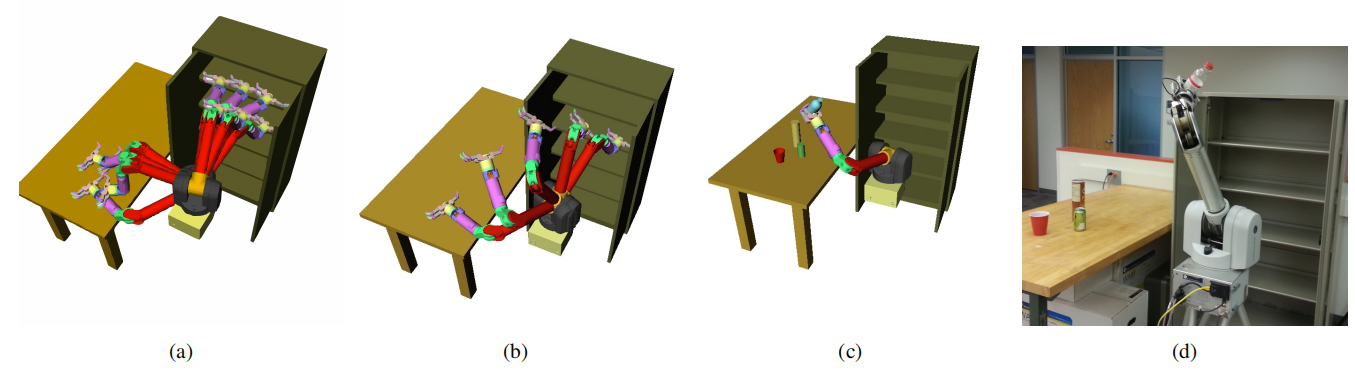
\includegraphics[scale=0.3]{论文1}

\caption{(a) Environment with 4 start robot arm configurations (on the table) and 6 end robot arm configurations (on the
cabinet shelves) used to generate a set of 24 unique planning problems. These planning problems entail displacing objects
from the table to the cabinet shelves. The plans are generated in OpenRAVE and executed on the real robot. (b) Example
of a successful plan generated by GPMP on one of the planning problems. This plan is used to move a milk bottle from
the table to a shelf in the cabinet in (c) simulation and (d) on the real WAM robot.}
\end{figure*}
and states) and then projected back onto just the states
using the matrix $M^T$
(see Eq. 36 below). The update rule
for this approach is derived from Eq. 33 as
\begin{align*}
\overline{\xi}&\leftarrow\overline{\xi}-\dfrac{1}{\eta}\mathcal{K}[\lambda\mathcal{K}^{-1}(\xi-\mu)+g]\\
\Longrightarrow M\overline{\xi}_w&\leftarrow M\overline{\xi}_w-\\
&\dfrac{1}{\eta}M\mathcal{K}_wM^T[\lambda M^{-T}\mathcal{K}_w^{-1}M^{-1}M(\overline{\xi}_w-\mu_w)+g]\\
\Longrightarrow\quad\overline{\xi}_w&\leftarrow\overline{\xi}_w-\dfrac{1}{\eta}\mathcal{K}_w[\lambda\mathcal{K}_w^{-1}(\overline{\xi}_w-\mu_w)+M^Tg]\\
\tag{36}
\end{align*}
where $\mathcal{K}_w$ is the kernel and $\mu_w$ is the mean of the trajectory
$\overline{\xi}_w$ with sparse set of states. We refer to this algorithm as
the Gaussian Process Motion Planner (GPMP).
\section{EXPERIMENTAL RESULTS}
We benchmarked GPMP against CHOMP, AugCHOMP,
STOMP, and TrajOpt by optimizing trajectories in OpenRAVE [27], a standard simulator used in motion planning [4],
[5], [8], [28]-[31], and validated the resulting trajectories
on a real robot arm. Our experimental setup consisted of a
table and a cabinet and a 7-DOF Barrett WAM arm which
was initialized in several distinct configurations. Figure 1 (a)
shows the start and end configurations of 24 unique planning
problems on which all the algorithms are tested.
For GPMP and AugCHOMP we employed a constantacceleration prior, i.e. white-noise-on-jerk model, $q'''(t)=w(t)$. (Recall that $w(t)$ is the process noise, see Eq. 6). For
simplicity we assumed independence between the degrees of
freedom (joints) of the robot. Following the form of LTVSDE in Eq. 6 we specified the transition function of any joint
$d \in D$,
\[
\Phi^d(t,s)=\begin{bmatrix}
1&(t-s)&\dfrac{1}{2}(t-s)^2\\
0&1&(t-s)\\
0&0&1
\tag{37}
\end{bmatrix}
\]
With the independence assumption, it follows that $\Phi(t, s) =
\text{diag}(\Phi^1
(t, s), \dots , \Phi^
D(t, s))$, and for all the states at $t_i
, i =
1 \dots N + 1$ we compute
\[
Q^d_i=\begin{bmatrix}
\dfrac{1}{2}\Delta t_i^5Q_c&\dfrac{1}{8}\Delta t_i^4Q_c&\dfrac{1}{6}\Delta t_i^3Q_c\\
\dfrac{1}{8}\Delta t_i^4Q_c&\dfrac{1}{3}\Delta t_i^3Q_c&\dfrac{1}{2}\Delta t_i^2Q_c\\
\dfrac{1}{6}\Delta t_i^3Q_c&\dfrac{1}{2}\Delta t_i^2Q_c&\Delta t_iQ_c
\end{bmatrix}
\]
\[
Q^d_i=\begin{bmatrix}
720\Delta t_i^{-5}Q_c^{-1}&-360\Delta t_i^{-4}Q_c^{-1}&60\Delta t_i^{-3}Q_c^{-1}\\
-360\Delta t_i^{-4}Q_c^{-1}&192\Delta t_i^{-3}Q_c^{-1}&-36\Delta t_i^{-2}Q_c^{-1}\\
60\Delta t_i^{-3}Q_c^{-1}&-36\Delta t_i^{-2}Q_c^{-1}&9\Delta t_i^{-1}Q_c^{-1}
\tag{38}
\end{bmatrix}
\]
where $\Delta t_i=t_i-t_{i-1}$. Similarly we compute $Q_i =\text{diag}(Q_i^1
, \dots, Q^D_i
)$ and $ Q_i^{-1}= \text{diag}((Q_i^{1})^{-1}
, \dots,(Q^D_i)^{-1})$.
The matrix $Q^{-1}$
(Eq. 13) can be built directly and efficiently
from the $Q_i^{-1}s$.

Both GPMP and AugCHOMP handle constraints (Eq 17)
in the same way as CHOMP. For AugCHOMP joint limits
are obeyed by finding a violation trajectory $\xi^v$
, calculated by
taking each point on the trajectory in violation and bringing
it within joint limits via a $L_1$ projection. It is then scaled by
the kernel such that it cancels out the largest violation in the
trajectory (see [5] for details),\footnote{For simplicity only positions in configuration space are considered while
calculating $\xi_v$
.}
\begin{equation*}
\overline{\xi}=\overline{\xi}+\mathcal{K}\xi^v
\tag{39}
\end{equation*}
Joint limits for GPMP are obeyed using a technique similar
to Eq. 36 applied to Eq. 39,
\begin{equation*}
\overline{\xi}_w=\overline{\xi}_w+\mathcal{K}_wM^T\xi^v
\tag{40}
\end{equation*}
For all algorithms except GPMP and AugCHOMP, trajectories were initialized as a straight line in configuration space.
For GPMP and AugCHOMP we found that initializing the
trajectory as a acceleration-smooth line yielded lower prior
cost at the start. The initialized trajectories were parameterized by 103 equidistant states. For GPMP 18 states were used
with $p = 5$ (103 states effectively), where $p$ is a parameter
that represents the number of points interpolated between
any two states during each iteration.
\begin{table*}[htp]
\centering
\caption{Results for 24 planning problems on the 7-DOF WAM arm. See text for details.}
\begin{tabular}{|c| c c c c c|}
\hline
&GPMP&AugCHOMP&CHOMP&STOMP&TrajOpt\\
\hline \hline
Problems Solved&24/24&24/24&18/24&10/24&23/24\\
Average Time to Success (s)&0.503&0.658&0.866&5.656&0.3737\\
Average Iterations to Success &22.125&22.958&38.378&82.837&6.087\\
\hline
\end{tabular}
\end{table*}
As observed in [5] the CHOMP trajectory can oscillate
between feasible and infeasible during optimization. This
behavior is observed in AugCHOMP and GPMP as well.
Therefore, with the exception of TrajOpt, all algorithms were
allowed to optimize for at least 10 iterations before checking
for feasibility. Once a feasible trajectory was discovered, the
solution was returned. We capped the optimization for these
algorithms at 250 iterations, after which, if a feasible solution
was not found, a failed trajectory was returned and the
problem was marked unsolved by the particular algorithm.

The results on the 24 arm planning problems for all the
algorithms are summarized in Table I.\footnote{Parameters for the benchmark were set as follows: For GPMP and
AugCHOMP, $Q_c=100$. For GPMP, AugCHOMP and CHOMP, $\lambda =
0.005, \eta = 1$. For STOMP, $k = 5$. For TrajOpt, coeffs = 20, dist pen
= 0.05.} Average time to
success was computed from successful runs, unsuccessful
runs were excluded. Since STOMP is stochastic in nature,
we ran the problem set on STOMP 5 times. The results for
STOMP reflect the aggregate of the 5 runs.
\section{DISCUSSION}
From the results in Table I we see that GPMP compares
favorably with recent trajectory optimization algorithms on
the benchmark. GPMP is able to solve all the 24 problems in
a reasonable amount of time, while solving for trajectories in
a state space 3 times the size of the state for all the other algorithms (with the exception of AugCHOMP). GPMP provides
a speedup over AugCHOMP by utilizing GP interpolation
during optimization, such that each iteration is faster without
any significant loss in the quality of the trajectory at the
end of optimization. This is illustrated in a comparison on
an example optimized trajectory obtained from GPMP and
AugCHOMP on the same problem (Figure 2).

GPMP and AugCHOMP are able to converge to better
solution trajectories (solve more problems) and do so faster
when compared to CHOMP. One advantage of these algorithms is that the trajectory is augmented with velocities and
accelerations. In contrast to CHOMP, where velocities and
accelerations are computed from finite differencing, velocities and accelerations in GPMP and AugCHOMP can be used
directly during optimization. This affects the calculation of
the objective cost and its gradient, resulting in better gradient
steps and convergence in fewer iterations.

Benchmark results show that TrajOpt is faster than our
approach and fails on only one of the problems. By formulating the optimization problem as sequential quadratic
programming (SQP), TrajOpt achieves faster convergence
with fewer iterations. However, GPMP offers several advantages over TrajOpt: the continuous representation allows
\begin{figure}[htp]
\centering
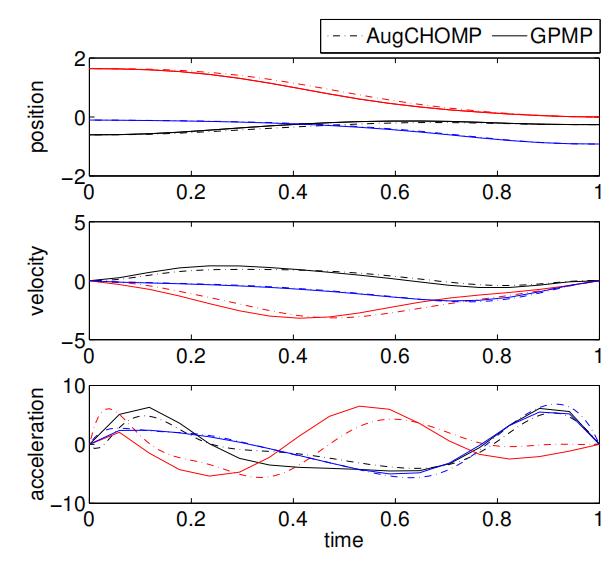
\includegraphics[scale=0.4]{论文2}
\caption{Comparison of an example optimized trajectory
(position, velocity and acceleration in configuration space)
obtained using GPMP (18 states) and AugCHOMP (103
states). The black, blue, and red lines, correspond to 3 of
the 7 degrees of freedom of the arm.
}
\end{figure}
GPMP to use only a few states to parameterize the trajectory, ensuring smoothness. GP interpolation can be used to
propagate obstacle cost from interpolated points to the states
during optimization, and also enables up-sampling the output
trajectory (ensuring smoothness and providing collision-free
guarantee) such that it is executable on a real system.

\section{CONCLUSIONS}
We have presented a novel approach to motion planning
using Gaussian processes for reasoning about continuous-time trajectories by optimizing a small number of states. We
considered trajectories consisting of joint positions, velocities, and accelerations sampled from a GP generated from
a LTV-SDE, and we provided a gradient-based optimization
technique for solving motion planning problems. The Gaussian process machinery enabled us to query the trajectory
at any time point of interest, which allowed us to generate
executable trajectories or reason about the cost of the entire
trajectory instead of just at the states. We benchmarked
our algorithm against various recent trajectory optimization
algorithms on a set of 7-DOF robotic arm planning problems,
and we validated our algorithms by running them on a 7-DOF
Barrett WAM arm. Our empirical results show GPMP to be
competitive or superior to competing algorithms with respect
to speed and number of problems solved.
\newpage
\bibliographystyle{ieeetr}
\cite{khatib1986real}
\cite{mabrouk2008solving}
\cite{chuang1998analytically}
\cite{ratliff2009chomp}
\cite{zucker2013chomp}
\cite{kalakrishnan2011stomp}
\cite{he2013multigrid}
\cite{schulman2013finding}
\cite{rasmussengaussian}
\cite{vijayakumar2005incremental}
\cite{kersting2007most}
\cite{nguyen2008learning}
\cite{sturm2009body}
\cite{deisenroth2011pilco}
\cite{tay2008modelling}
\cite{barfoot2014batch}
\bibliography{cankaowenxian}
\end{document}
